\chapter{Lecture 14: Rouché's Thm. \& Fundamental Thm. of Algebra}

\section{Last Time: Counting zeroes and poles of analytic functions}

\begin{proposition}
    We say:
    \begin{itemize}
        \item[]
        \item $h$ analytic in $D$, except finite number of poles $z_1, \ldots, z_n$.
        \item $\gamma$ piecewise $C^1$ closed curve, positively oriented, inside$(\gamma) \subset D$ avoiding zeroes and poles of $h$.
    \end{itemize}
    Then
    \begin{align*}
        (A) \quad & \frac{1}{2\pi i} \int_{\gamma} \frac{h'(z)}{h(z)} \, dz = \text{\# of zeroes of $h$ inside $\gamma$} - \text{\# of poles of $h$ inside $\gamma$}. \\
        (B)\quad  & \text{Argument Principle}                                                                                                                         \\
                  & \frac{1}{2\pi i} \left\{\text{Total change in Arg}(h(z))_{\gamma} \text{ as } z \text{ traverses} \right\}                                        \\
                  & = \text{\# of zeroes of $h$ inside $\gamma$} - \text{\# of poles of $h$ inside $\gamma$}.
    \end{align*}

\end{proposition}

\begin{theorem}
    [Rouche's Theorem]
    Suppose $f, g$ are analytic on $D$, $\gamma$ a curve in $D$ (piecewise $C^1$, simple, closed).\\
    if $|f(z) + g(z)| < |f(z)| \quad \forall z \in \gamma$ then $f$ and $g$ have the same number of \underline{zeroes} inside($\gamma$) (counting multiplicities).
\end{theorem}

\begin{proof}
    Neither $f$ nor $g$ have zeroes on $\gamma$.\\
    Suppose $f,g$ have zeroes of multiplicity $k$ at $z_0$. Then (by definition of zero multiplicity):
    \begin{align*}
        \tilde{f} = \frac{f(z)}{(z-z_0)^k}, \quad \tilde{g} = \frac{g(z)}{(z-z_0)^k}
    \end{align*}
    are analytic on $D$ (even at $z_0$). And $\tilde{f(z_0)} \neq 0 \neq \tilde{g(z_0)}$, and
    \begin{align*}
        |\tilde{f}(z) + \tilde{g}(z)| < |\tilde{f}(z)| \quad \forall z \in \gamma
    \end{align*}
    So the number of zeroes of $\tilde{f}$ (or $\tilde{g}$) inside $\gamma$ is
    \begin{align}
        \text{\#zeroes}(f)     & = \text{\#zeroes}((z-z_0)^k) + \text{\#zeroes}(\tilde{f}) = k + \text{\#zeroes}(\tilde{f}) \\
        \text{\#zeroes}(f) - k & = \text{\#zeroes}(\tilde{f})                                                               \\
        \text{\#zeroes}(g) - k & = \text{\#zeroes}(\tilde{g})
    \end{align}
    % \begin{align*}
    %     \text{\#zeroes}(\tilde{f} - \frac{k}{(z-z_0)^k}) = \text{\#zeroes}(f) - k  = \text{\#zeroes}(\tilde{g}) = \text{\#zeroes}(\tilde{g} - \frac{k}{(z-z_0)^k}) - k
    % \end{align*}
    % Because:
    % \begin{align*}
    %     (f) - k                         & = 0 \\
    %     \tilde{f} - \frac{k}{(z-z_0)^k} & = 0
    % \end{align*}
    So the number of zeroes of $\tilde{f}$ (or $\tilde{g}$) inside $\gamma$ is the number of zeroes of $f$ minus $k$
    So it suffices to assume $f,g$ have no common zeroes with $\gamma$.\\
    Also, if $\tilde{f}(z_0) = 0 = \tilde{g}(z_0)$ then $|f(z_0) + g(z_0)| < |f(z_0)|$ is impossible anyways.\\
\end{proof}

\begin{example}
    Consider $\frac{g}{f}$ Which has zeroes at zeroes of $g$ and poles at zeroes of $f$.\\
    \underline{and: } $|\frac{g}{f} + 1| = |\frac{g+f}{f}| < 1$ on $\gamma$.\\
    Consider the curve $\frac{g}{f} (\gamma)$
    \begin{figure}[h]
        \centering
        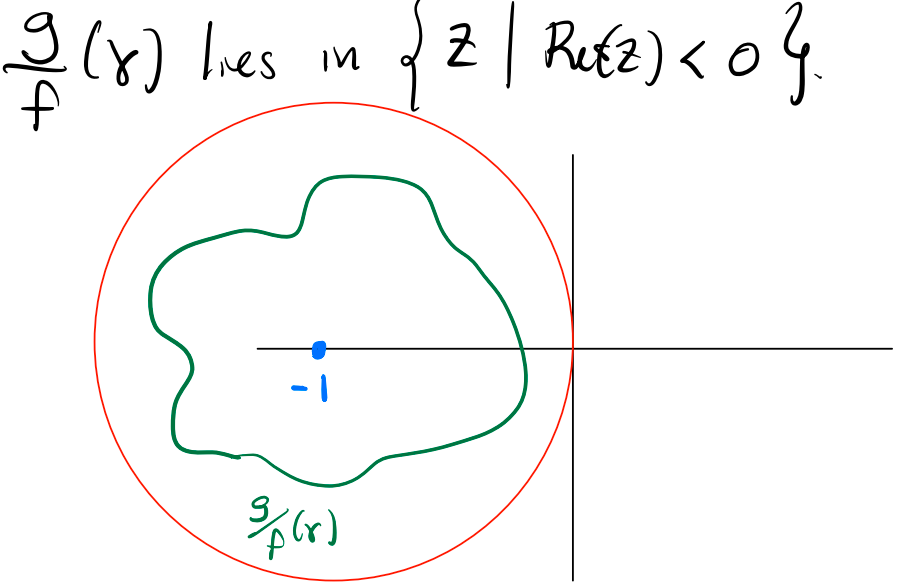
\includegraphics[width=0.8\textwidth]{LECTURE_14/gamma.png}
        \caption{Curve $\frac{g}{f} (\gamma)$}
    \end{figure}
    So, total change in argument of $\frac{g}{f}$ on $\gamma$ is \underline{zero}.\\
    So by the Argument Principle:
    \begin{align*}
        \text{\#zeroes}(\frac{g}{f}) = \text{\#poles}(\frac{g}{f}) = \text{\#zeroes}(f) = \text{\#poles}(g)
    \end{align*}

\end{example}

\begin{example}
    Show that all zeroes of the polynomial $p(z) = 3z^3 - 2z^2 + 2iz -8$ lie in the annulus $1 < |z| < 2$.\\
\end{example}

\begin{proof}
    \textbf{We apply Rouche's Theorem:}
    \textbf{Step 1:} Show that $p(z)$ has no zeroes inside $|z| = 1$.\\
    Consider the claim:
    \begin{align*}
        |p(z) + 8| < |8| \quad \forall z \in |z| = 1
    \end{align*}
    Let's show that it's true:

    \begin{align*}
        |p(z) + 8| & = |3z^3 - 2z^2 + 2iz|       \\
                   & \leq 3|z|^3 + 2|z|^2 + 2|z| \\
                   & = 3 + 2 + 2 = 7 < 8
    \end{align*}
    And therefore, the number of zeroes of $p$ in $|z| \leq 1$ is equal to the number of zeroes of 8, which is 0.\\
    \textbf{Step 2:} We expect an order 3 polynomial to have 3 zeroes, because there are none inside $|z| = 1$ we expect all 3 to be in $1 < |z| < 2$.\\

    Consider:
    \begin{align*}
        f(z)          & = -3z^3                                                                 \\
        |p(z) + f(z)| & < |f(z)| \text{ on } |z| = 2                                            \\
        |p(z) + f(z)| & = |-2z^2 + 2iz - 8|                                                     \\
                      & \leq 2|z|^2 + 2|z| + 8 = 2(4) + 2(2) + 8 = 20 < 3 \cdot 8 = 24 = |f(z)|
    \end{align*}

    So $p(z)$ has 3 zeroes in $1 < |z| < 2$ by Rouche's Theorem.\\
\end{proof}

\begin{theorem}
    [The Fundamental Theorem of Algebra]
    If you have a polynomial $p(z) = a_n z^n + a_{n-1} z^{n-1} + \ldots + a_1 z + a_0$ with $a_n \neq 0$ and $a_n, z \in \mathbb{C}$ then $p(z)$ has exactly $n$ zeroes in $\mathbb{C}$ (counting multiplicities).
\end{theorem}

\begin{proof}
    Let's compare $p(z)$ with $z^n$ on $|z| = R$ for $R$ large enough.\\
    \begin{align*}
        |p(z) - z^n| & \leq n\max_{0 \leq i \leq n - 1} |a_i||z|^i        \\
                     & = n\max_{|z| = R}^{n-1} |a_i| R^i \leq R^n = |z|^n
    \end{align*}
    So:
    \begin{align*}
        |p(z) - z^n| & < |z^n| \quad \forall |z| = R \quad \text{ for } R \text{ large enough}
    \end{align*}
    \underline{Rouche's} Theorem implies that $p(z)$ and $z^n$ have the same number of zeroes in $|z| < R$ for $R$ large enough.\\
\end{proof}
